\documentclass[10pt,letterpaper]{article}

\providecommand{\main}{.}
\usepackage{cogsci}
\usepackage{pslatex}
\usepackage{graphicx}
\usepackage{multicol}
\usepackage{blindtext}
\usepackage{tablefootnote}
\usepackage{hyperref}
\usepackage{tipa}
\usepackage[style=apa]{biblatex}
\DeclareNameAlias{sortname}{family-given}
\addbibresource{qp1.bib}
\usepackage{gb4e}

\graphicspath{{\main/figures/}{figures}}

\title{`Sally the Congressperson': Individuals' Ideologies Modulate the Production of Gender-Neutral Role Nouns in English}

\author{{\large \bf Brandon Papineau (branpap@stanford.edu)} \\
	Department of Linguistics, Margaret Jacks Hall, Bldg. 460\\
	Stanford, CA, 94305 USA}

%\\\\	
%{\large \bf Judith Degen (jdegen@stanford.edu)} \\
%Department of Linguistics, Margaret Jacks Hall, Bldg. 460\\
%Stanford, CA, 94305 USA\\\\	
%{\large \bf Robert J. Podesva (podesva@stanford.edu)} \\
%Department of Linguistics, Margaret Jacks Hall, Bldg. 460\\
%Stanford, CA, 94305 USA

\begin{document}
	
	\maketitle
	
	\begin{abstract}
		Language and society are inextricably linked, such that our views and knowledge of the social world can influence the ways in which we process and produce language, a line of thinking which has garnered great attention in both the sociolinguistic and psycholinguistic literatures. This is particularly salient in the realm of gender, where we often linguistically negate stereotypical assumptions about the gendered nature of particular social occupations, such as in the case of `male nurse' \parencite{hellinger2001english}. Recent scholarship has also found that the expectations regarding a real-world event as held by an individual can modulate that individual's production of gendered terms as they relate to that event \parencite{von2020implicit,pozniak2021failures}. We extend this line of thinking by examining the role of individual and group ideologies towards gender on the production of gender-neutral role titles. Using a forced-choice production task, we find that self-identified Democrats produce a higher proportion of gender-neutral terms than Republicans, and that Democrats' productions are sensitive to the ideologies of individuals, while Republicans' are not. Finally, we find that female names are more likely to elicit subsequent gender-neutral productions, regardless of participant political party.  
		
		\textbf{Keywords:} 
		language and gender; language production; language and politics; morphology
	\end{abstract}
	
	
	\section{Introduction}
	Linguists have long been aware that individuals' and groups' orientations towards and away from particular identities, ideologies, or social groups influence the ways in which they engage with and employ their linguistic systems. This line of thinking can be traced back over 50 years, to Labov's seminal 1963 paper, which found that the residents of Martha's Vineyard produced diphthongs whose realizations were modulated by (or indexical of) their relationships to the island and its changing economic and cultural realities. More contemporarily, \textcite{podesva2015country} asserts that individuals from Redding participate in the California Vowel Shift to varying degrees, which are themselves a function of their orientation towards `town' (urban) or `country' (rural) identities. \par 
	Beyond highly local identities, though not entirely removed from them, recent scholarship has linked the belonging of individuals to supralocal political groups as a predictor of linguistic production and perception. \textcite{hall2010indexing} found that Republicans in the United States House of Representatives were more likely to produce /\ae/ in the second syllable of \textit{Iraq} than their Democratic counterparts, who were more likely to produce /a:/. On the other hand, however, \textcite{hall2020breksit} find no such correlation in the production or perception of the voicing of the word-medial consonant cluster in the portmanteau \textit{Brexit}. Rather, the voiced variant /gz/ appears to index `whoever I think is wrong', regardless of what political belief the individual in question. So while not a predictor of linguistic production itself, the \textit{perception} of the cluster in \textit{Brexit} appears to be driven by political and personal ideologies.\par 
	On the experimental front, there is a burgeoning landscape of literature investigating the relationship between ideology and personal beliefs as they relate to the processing and production of gendered language, which builds on previous work examining the relationship between societal expectations and reading times on gender-anomalous coreferents, such as \textit{he} for \textit{flight attendant} or \textit{she} for \textit{electrician} \parencite{foertsch1997search,duffy2004violating}. \textcite{von2020implicit} found that, in the context of the United States 2016 presidential election, participants' beliefs on whether or not Hillary Clinton would win the presidency had no effect on the production of \textit{she} as a coreferent pronoun with `the future president', and that `she' induced a processing penalty when read in a context in which it was coreferent with `the future president'. They did find that, in the context of the 2017 British General Election, coreferential \textit{she} was produced more frequently than \textit{he} when coreferential with the future Prime Minister, but that there was no such processing bonus for \textit{she} over \textit{he}, indicating lingering sexist beliefs in the realm of language processing, even when the incumbent (Theresa May) was female. Similarly, \textcite{pozniak2021failures} found that respondents who believed that female candidates would win in the 2020 Parisian and Marseille municipal elections were more likely to produce feminine-marked coreferential terms (both nouns and pronouns), but that masculine-marked forms were still dominant in both locales. \par 
	While these studies present valuable insights into the ways in which individuals' beliefs about gender and specific referents influence their productions of gendered co-referents, they are limited in their generalizability in that they pick out real-world referents and events. Moreover, the diagnostic used to characterize individuals' beliefs specifically targets their predictions about real-world events, rather than their general ideologies towards gender. In order to investigate the question of how individuals' ideologies towards social categories such as gender may impact the production of gendered language, we conduct a forced-choice production task in which participants are tasked with assigning coreferential role nouns \parencite{misersky2014norms} marked for morphological gender to gendered characters in short fill-in-the-blank tasks. Such terms are one of only a small number of corners of the English language in which gender is still marked, by way of compounding (e.g. \textit{congress-man}, \textit{congress-woman}, \textit{congress-person}), though this is typically described as a manifestation of lexical, rather than grammatical, gender \parencite{kastovsky2011inflectional,hellinger2001english}. We examine these productions as a function of social ideology according to \textcite{baber2006social}'s Social Roles Questionnaire, and also as a function of political alignment. \par
	
	\section{Experiment}
	
	\subsection{Methods}
	\subsubsection{Participants} 301 participants were recruited using Prolific. 100 Democrats and 100 Republicans were recruited initially, in order to maintain a political balance. All participants additionally self-identified as L1 English speakers and as having been born and in the United States, and all lived in the United States at the time of participation. None of the participants had participated in the pilot study or in any other study related to the present project. An additional 100 male-identifying participants were subsequently recruited do to a significant gender imbalance in the initial participant population (13.4\% male-identifying participants in the original population), as a result of an influx of female participants after Prolific went viral on social media app TikTok \parencite{charalambides2021}. The final gender-political distribution (after exclusions, see below) is provided in Table 1.\par
	Participants were paid at a rate of \$15-\$16 an hour for their participation in the study, regardless of whether or not their data was used in the final analysis.
	
	\begin{table}[!ht]
		\begin{center} 
			\caption{Participants by Gender and Political Orientation} 
			\label{sample-table} 
			\vskip 0.12in
			\begin{tabular}{llll} 
				\hline
				  &  Democrat & Republican & Centrist\tablefootnote{These participants were recruited as either Democrats or Republicans, but reported a centrist identity in the post-experimental questionnaire} \\
				\hline
				Female &  82 & 62 & 25 \\
				Male & 42 & 46 & 10 \\
				Other & 4 & 0 & 0 \\
				Decline to state & 1 & 0 & 1 \\
				\hline
			\end{tabular} 
		\end{center} 
	\end{table}
	
	\subsubsection{Stimuli \& Procedure} All items in the experiment consisted of a complete sentence missing a single word. Participants were then provided with either two or three words which could complete the sentence by filling in the blank, and were asked to select the word which best did that. There were a total of 80 trials, with 20 critical items and 60 filler items.\par 
	Critical items took the form ``[NAME] is a [blank] from [STATE]", where the blank was one of 14 social roles which shows a ternary distinction in its gender marking (e.g. \textit{congressman}, \textit{congresswoman}, \textit{congressperson}). An additional six critical items making only a binary distinction (e.g. \textit{villain} vs. \textit{villainess}) were also tested, but the results of these items are not reported on here. The twenty most popular male and female names were selected from the lists of most popular names for boys and girls in 1998 according to the Social Security \textcite{socialsecurity}. Names which appeared within the top 100 entries on both lists (e.g. Taylor, Ryan) were excluded, in order to ensure that the names used in the experiment were sufficiently socially gendered along binary lines. These names were randomized between participants, with no participant seeing the same name more than once. States and activities were randomized at the stimuli creation stage so that they remained constant for all participants.\par 
	Filler items took one of two forms; semantic fillers and grammatical fillers. Semantic fillers had no prescriptively correct answer, and employed items from the same semantic field (1) or made use of common idioms or sayings (2). Some of these questions also dealt specifically with social and occupational titles and adopted the same syntactic frame as the critical items, in order to distract from the salience of gender in the critical items (3). 
	
	\begin{exe}
		\ex That's the cutest (horse/Lusitano/equine) I have ever seen!
		\ex The (customer/parent/child) is always right.
		\ex Revati is a (writer/journalist/author) from India.
	\end{exe}

	Grammatical fillers, on the other hand, had prescriptively correct answers, and employed grammatical processes such as demonstrative selection (3), verb agreement (4), or preposition selection (5), among others. These items served a secondary purpose as attention check questions, and participants who answered incorrectly on more than 20\% of these questions were excluded from analysis (25 participants; see below).
	
	\begin{exe}
		\ex She is typing on (\textbf{the}/these/those) computer.
		\ex Katherine (\textbf{sang}/song/sing) that song beautifully. 
		\ex They are they eating their soup (between/\textbf{with}/at) a spoon.
	\end{exe}

	All response possibilities, regardless of type (filler or critical) were shuffled between participants to control for possible ordering effects of presented options. As such, the examples in (1)-(6) are not necessarily indicative of the orders in which options were presented to participants. Similarly, all 70 trials were randomized between participants, after which they moved to the post-experimental phase of the study. 

	\subsubsection{Post-Experimental Survey} In order to assess the participants' ideologies towards gender, we employ the Social Roles Questionnaire developed by \textcite{baber2006social}. This survey consists of 13 questions which are designed to elicit both implicit and explicit ideologies about gender, including the notions of gender as an immutable fact vs gender as a social construct (what Baber and Tucker term `gender transendence'), as well as about the societal roles performed by the (binary) genders (`gender linking').\par 
	Each of the 13 questionnaire items was presented alongside a sliding scale from `strongly disagree' to `strongly agree', which corresponded to numerical values of 0 and 100, respectively. The questions related to `gender linking' were inversely coded. Participants were then assigned a gender ideology score from 0 to 100 by taking the mean of their individual responses; the closer to 0 a participant is, the more open-minded their approach to gender, and the closer to 100, the more conservative or traditional their view of gender.\par 
	Finally, participants filled out an optional post-experimental demographic survey. This included questions about their own gender, political affiliations, and age. The full survey is available online as part of the supplementary materials.
	
	\subsection{Results}
	\subsubsection{Exclusions} 25 participants were excluded for not meeting the 80\% threshold for accuracy on the attention check questions. This yielded a total of 5,480 observations included in the final analysis.
	
	\subsubsection{Response Gender by Political Party}
	Responses were coded according to the gender which was seen in the target sentence; male names were coded as `male' stimuli gender and female names as `female' stimuli gender. We found that participants who identified as Democrats produced higher proportions of gender-neutral role titles than Republicans in both the male ($\beta$=-0.128, \textit{SE}=0.023, \textit{t}=-5.547, \textit{p}$<$0.0001) and female ($\beta$=-0.098, \textit{SE}=0.023, \textit{t}=-4.222, \textit{p}$<$0.0001) stimuli gender conditions, as highlighted in Figure 1.
	
	\begin{figure}[ht!]
		\centering
		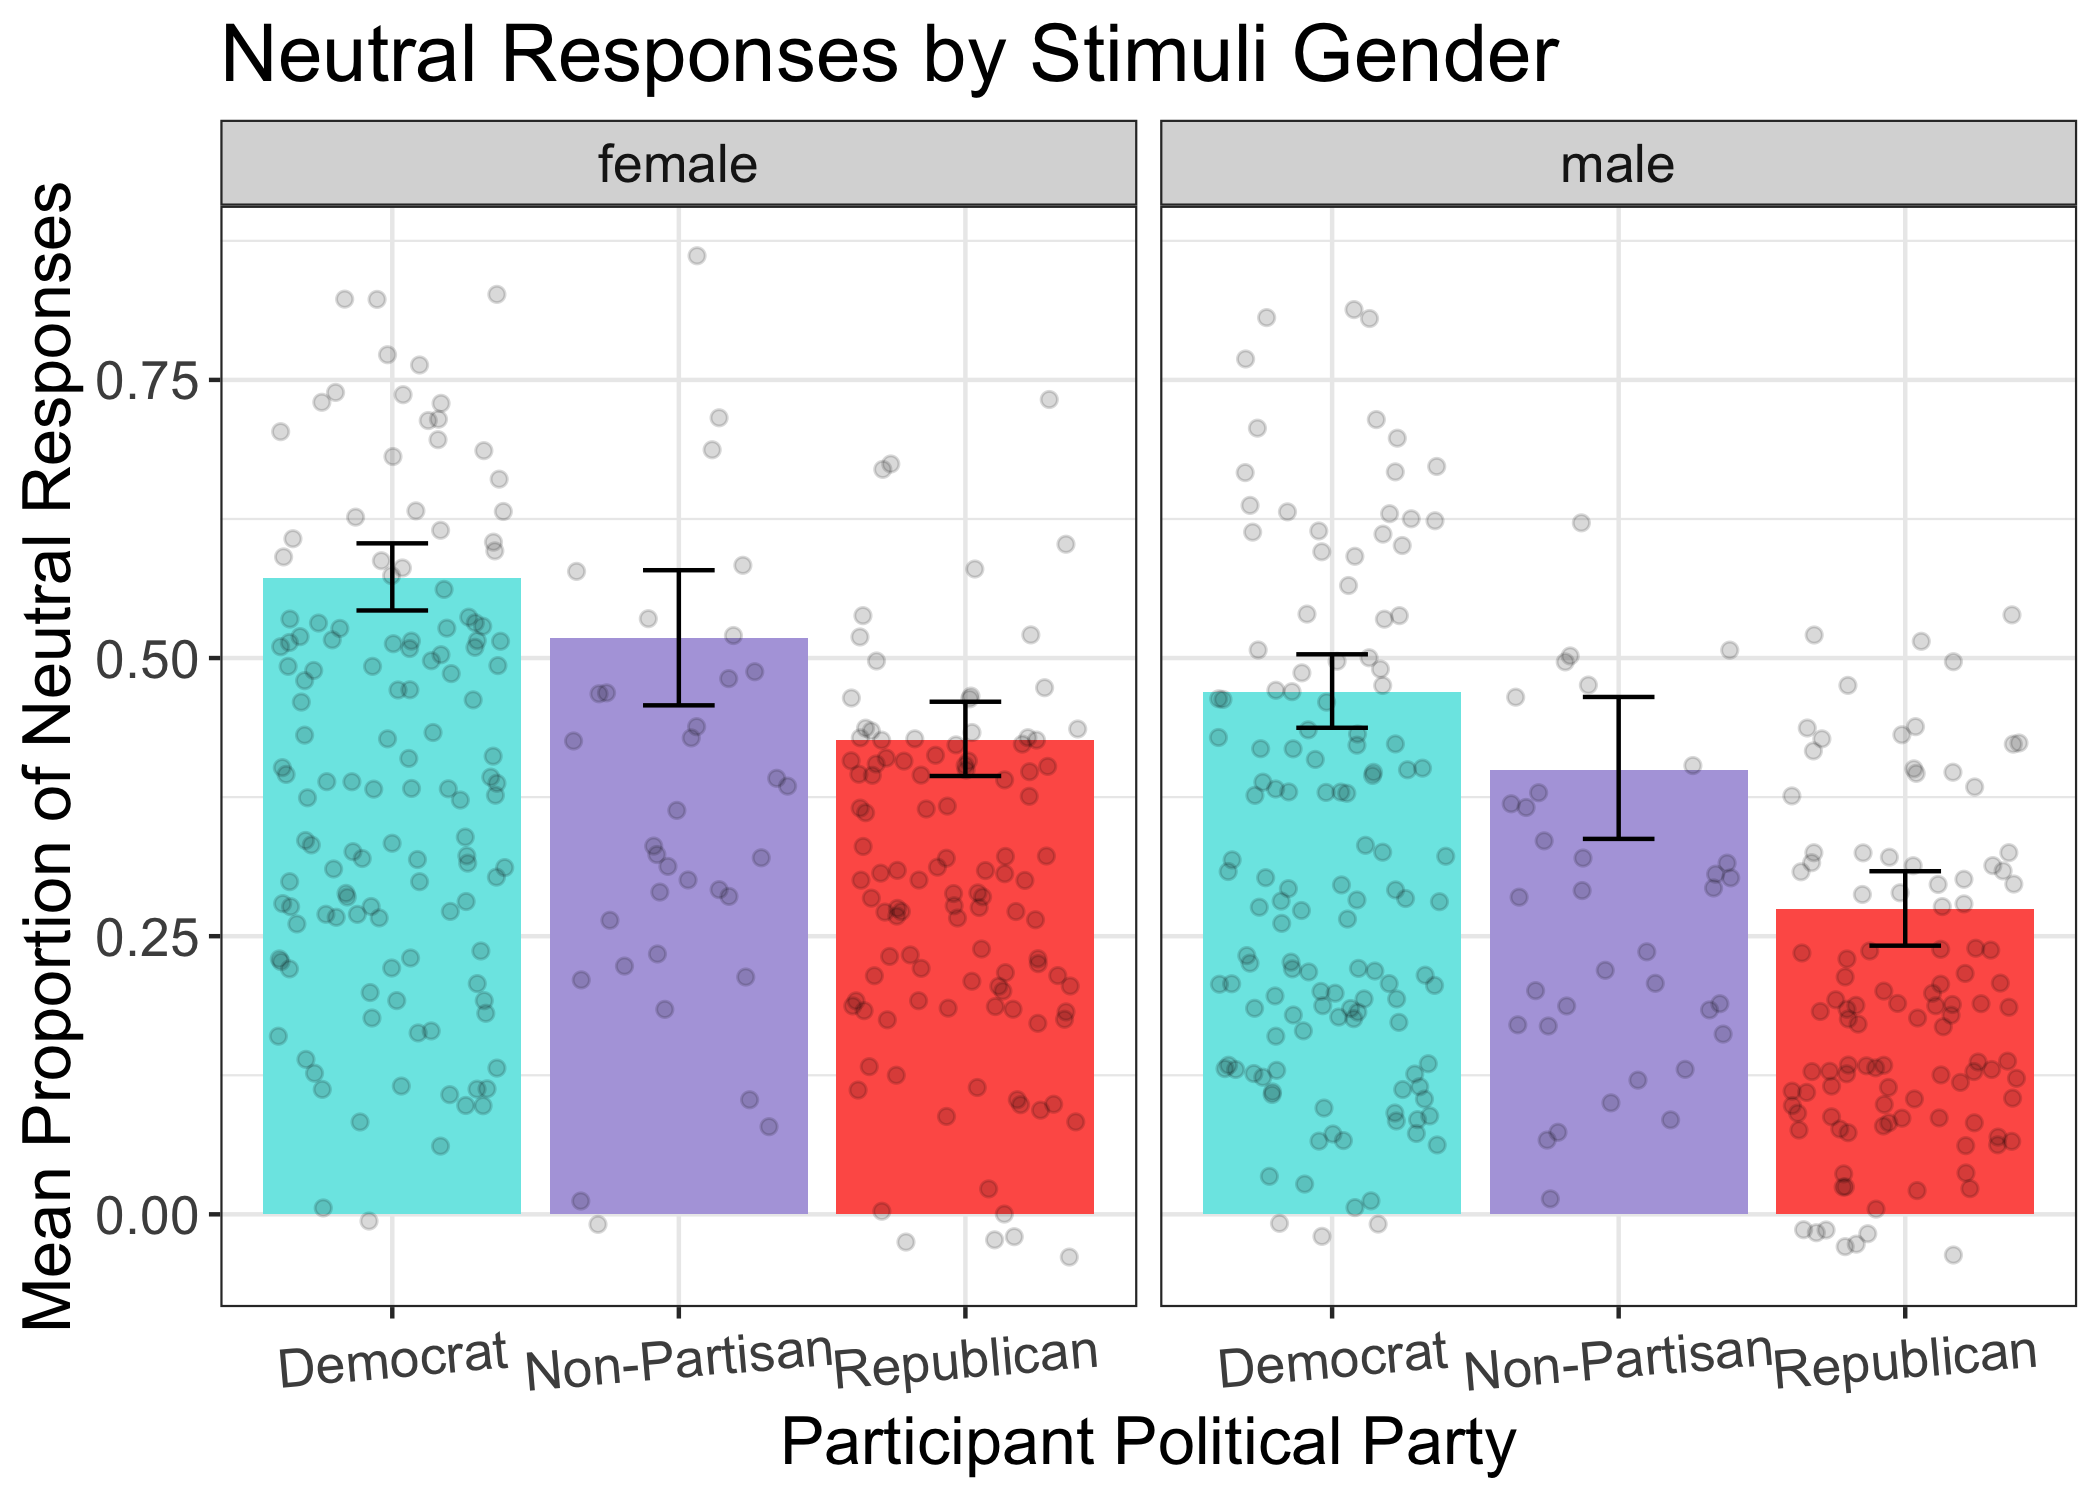
\includegraphics[scale=0.115]{prod_neutral_poli_bar_nonmean.png}
		\caption{Proportion of response genders by political party, faceted by gender of name in vignette seen.}
		\label{prod-box}
	\end{figure}
	
	Figure 2 shows the second principal finding of the role of stimuli gender; we observe that participants, regardless of political party, had higher rates of gender-neutral coreferential title productions when those titles were coreferential with female names than with male names  ($\beta$=-0.077, \textit{SE}=0.018, \textit{t}=-4.408, \textit{p}$<$0.0001). 
	
		\begin{figure}[ht!]
		\centering
		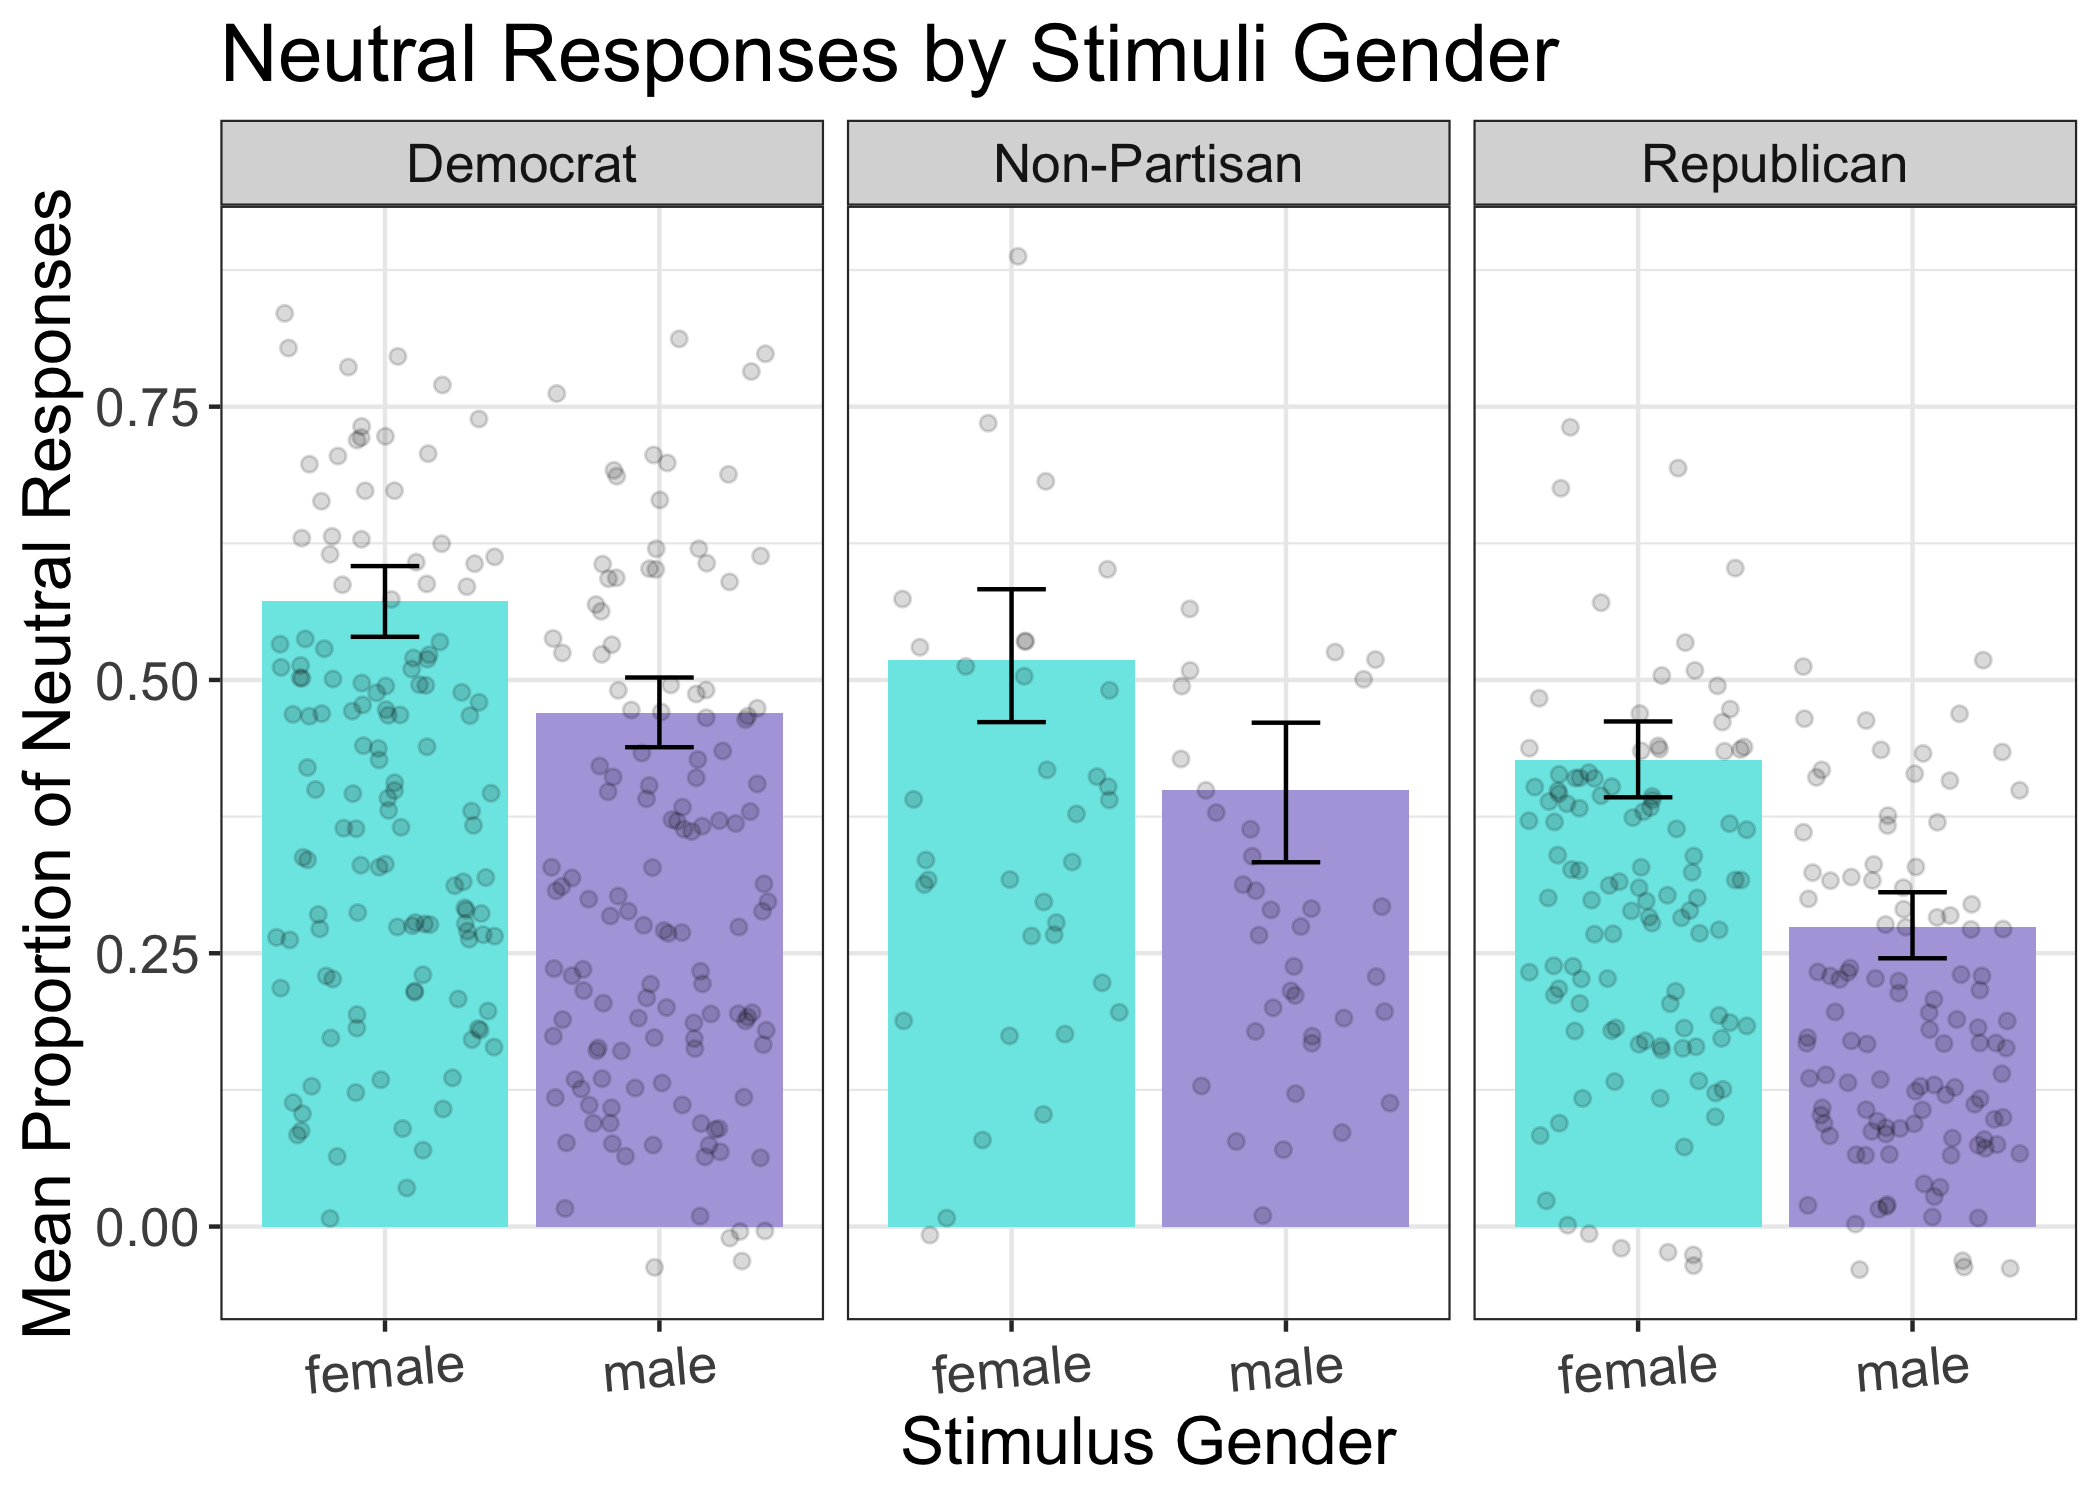
\includegraphics[scale=0.115]{prod_neutral_gender_bar_nonmean.png}
		\caption{Average proportion of neutral responses as a function of gender ideology, faceted by political alignment.}
		\label{prod-neutral-poli-box-gender}
	\end{figure}
	
	\subsubsection{Response Gender by Political Party \& Individual Ideology}
	We turn now to the more fine-grained issue at hand, which is the role of individuals' ideologies about gender in their production of gender-neutral forms. Highlighted in Figure 3, we find that ideology does have a significant effect on the proportion of gender-neutral coreferential role titles produced, but that this is driven by Democrat-identifying participants ($\beta$=-.006, \textit{SE} = 0.001, \textit{t}=-5.345, \textit{p}$<$.0001), as Republican-identified participants show no such significant effect ($\beta$ = 0.000, \textit{SE}=0.000, \textit{t}=-0.382, \textit{p}$<$0.703). That is, Democrats with more conservative gender ideologies produce lower proportions of gender-neutral terms than Democrats with more progressive gender ideologies, while Republicans rates of gender-neutral productions stay relatively stable, regardless of the individual's ideology towards gender.
			
	\begin{figure*}[ht!]
	\centering
	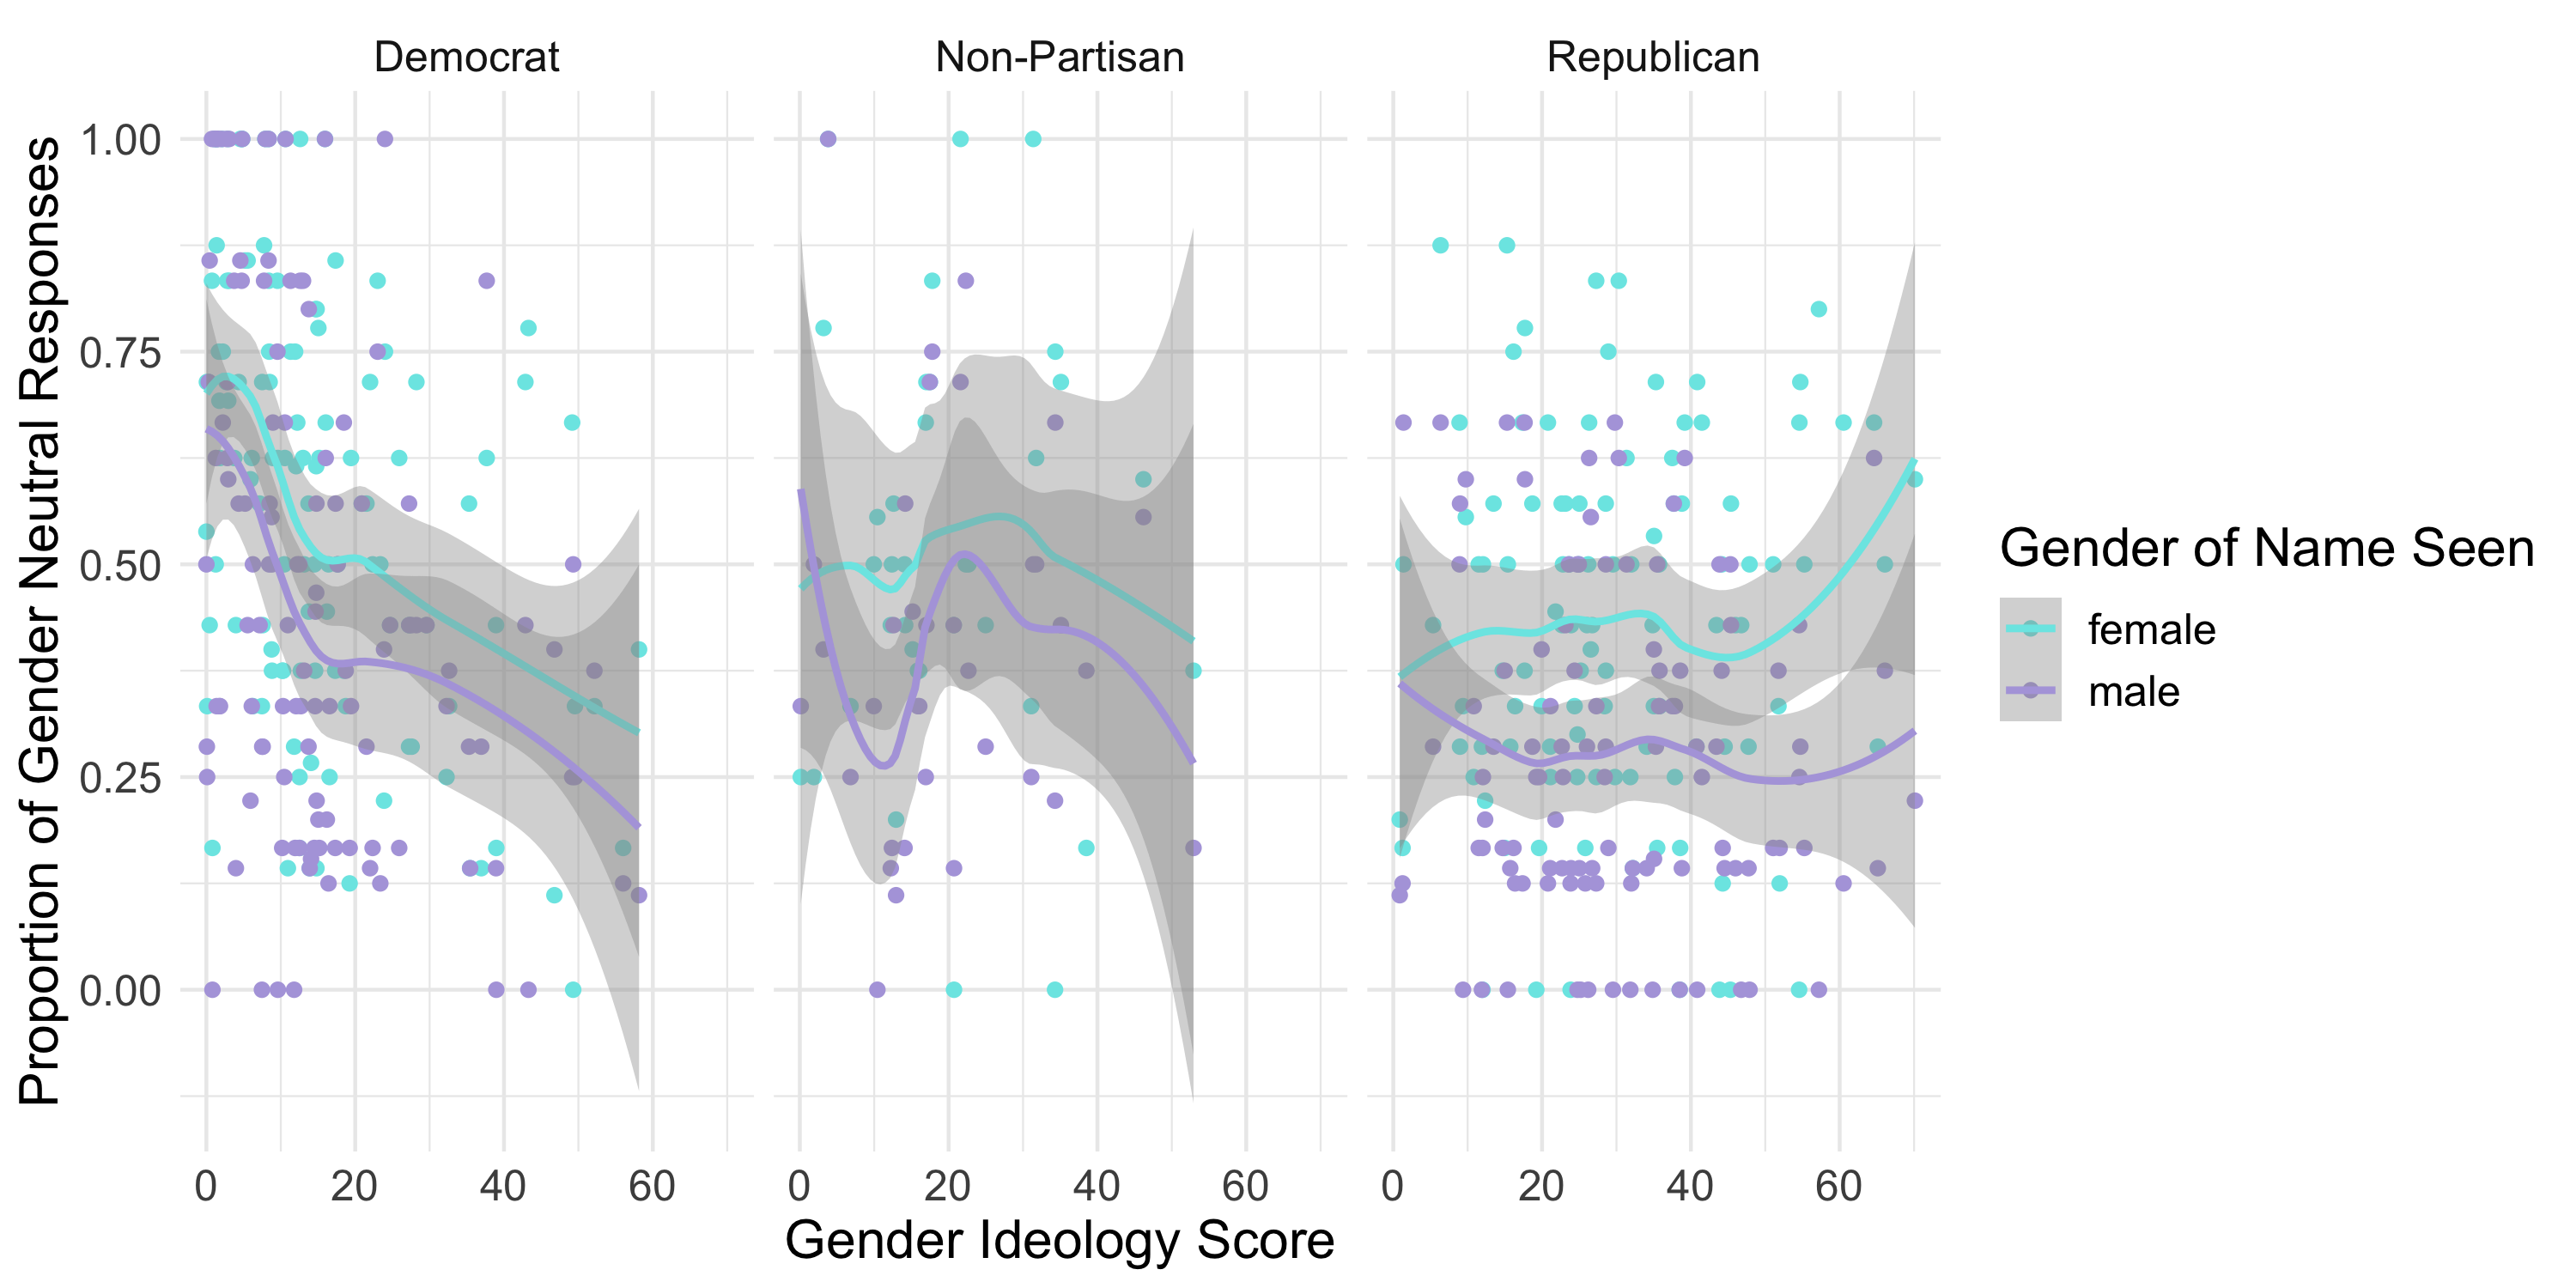
\includegraphics[scale=0.15]{prod_neutral_poli.png}
	\caption{Average proportion of neutral responses as a function of gender ideology, faceted by political alignment.}
	\label{prod-neutral-poli}
\end{figure*}
	\section{General Discussion}
	
	\subsection{The Female Effect in Gender Neutral Productions}
	Of note in the findings is that female coreferential names are consistently more likely to be assigned gender-neutral role titles than their male counterparts. This is perhaps surprising, as, with the singular exception of \textit{flight attendant}, all of the neutral forms in our norming study were evaluated as either equally likely to be of either gender, or significantly more likely to be describing a male referent\footnote{The full results of the norming study are available in the online supplementary materials}. These findings are presented in Figure 4.
	
	\subsection{The Role of Political Ideology in Gender Neutral Productions}
	
	\section{Acknowledgments}
	
	\section{Supplementary Material}
		Supplementary materials, including details related to the norming study and unreported processing studies, can be found at \url{https://branpap.com/qp1-supplementary-materials}.
		
	\nocite{labov1963social}
	\printbibliography
	
	
\end{document}